% This example is meant to be compiled with lualatex or xelatex
% The theme itself also supports pdflatex
\PassOptionsToPackage{unicode}{hyperref}
\documentclass[aspectratio=1610, 12pt]{beamer}

% Load packages you need here
\usepackage[english]{babel}

\usepackage{csquotes}
    
\usepackage{xcolor}
\usepackage{listings}
\usepackage{amsmath}
\usepackage{amssymb}
\usepackage{mathtools}
\usepackage{hyperref}
\usepackage{bookmark}
\usepackage{array}
\usepackage{tikz}
\usetikzlibrary{positioning,shapes,fit}
\usetikzlibrary{calc}
\usetikzlibrary{arrows.meta}
\usepackage{varwidth}


% load the theme after all packages

\usetheme[
  showtotalframes % show total number of frames in the footline
]{tudo}


\lstdefinestyle{cstyle}{
	belowcaptionskip=1\baselineskip,
	breaklines=true,
	frame=single,
	xleftmargin=\parindent,
	language=C,
	escapeinside={(*@}{@*)},
	showstringspaces=false,
	basicstyle=\footnotesize\ttfamily,
	keywordstyle=\bfseries\color{green!40!black},
	commentstyle=\itshape\color{purple!40!black},
	identifierstyle=\color{gray},
	stringstyle=\color{orange},
}
% Put settings here, like
\makeatletter
\newcommand{\thickhline}{%
	\noalign {\ifnum 0=`}\fi \hrule height 1pt
	\futurelet \reserved@a \@xhline
}
\newcolumntype{"}{@{\hskip\tabcolsep\vrule width 1pt\hskip\tabcolsep}}

\definecolor{preload}{RGB}{184, 17, 17} 
\definecolor{mm1}{RGB}{189, 117, 28}
\definecolor{mm2}{RGB}{130, 22, 87}
\definecolor{mm3}{RGB}{15, 112, 57}


\title{MNIST Training for BNN}
\author[Diep, Köhler, Naumann]{Jack Diep, Florian Köhler, Yannick Naumann}
\institute[BNN-Training]{Design Your Own CPU - Design of Embedded Systems}
\titlegraphic{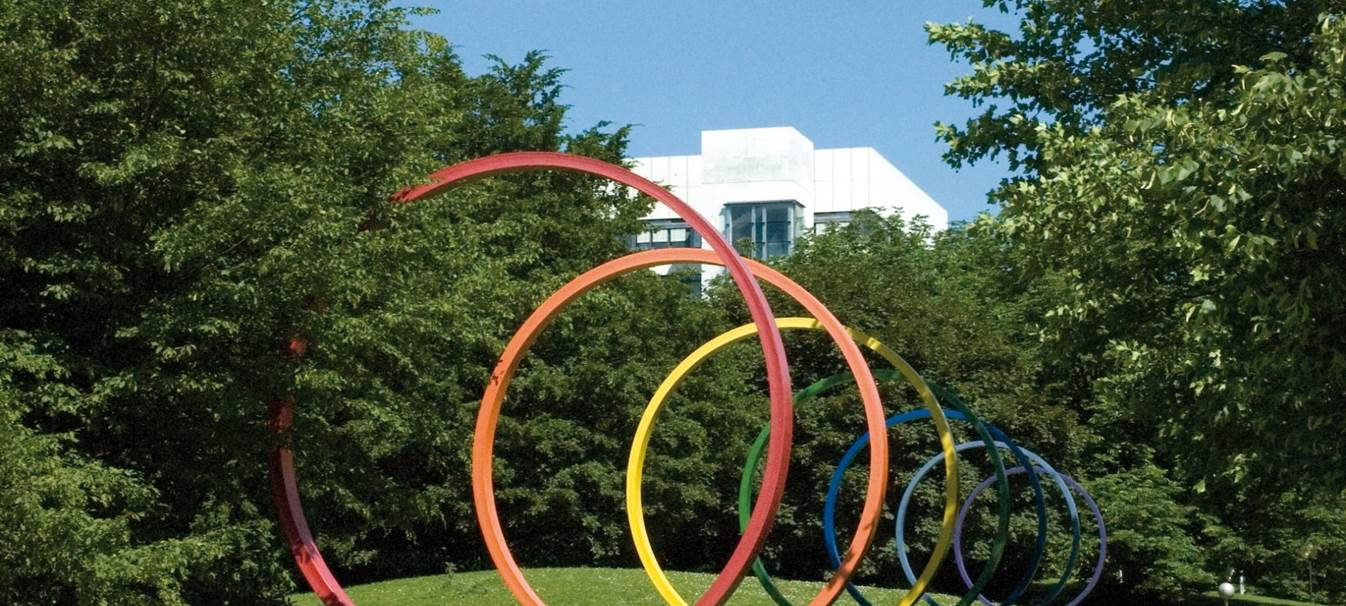
\includegraphics[width=0.675\textwidth]{images/tudo-title-2.jpg}}

\setbeamertemplate{section in toc}{%
	{\color{tugreen}\inserttocsectionnumber.}~\inserttocsection}
\setbeamercolor{subsection in toc}{bg=white,fg=structure}
\setbeamertemplate{subsection in toc}{%
	\hspace{1.2em}{\color{tugreen}\rule[0.3ex]{3pt}{3pt}}~\inserttocsubsection\par}



\begin{document}


\maketitle




\begin{frame}{Content}
	\tableofcontents


\end{frame}
\section{Neural Networks}

\subsection{What is a neural network?}

\begin{frame}
	\centering
	\vfill
	\textbf{\Large What is a neural network?}
	\vfill
\end{frame}

\begin{frame}
	\frametitle{What is a neural network?}

	\begin{itemize}
		\item<+-> The heart of deep learning
		\item<+-> Classify given data

		\emph{e.g. speech or image recognition}

		\item<+-> Rely on training data
	\end{itemize}

\end{frame}

\begin{frame}{What is a neural network?}
	\centering
	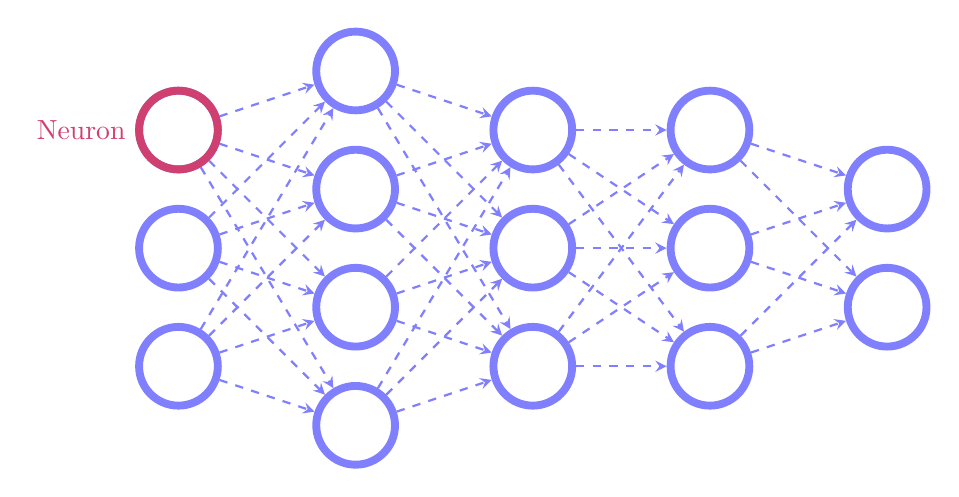
\begin{tikzpicture}[x=2.25cm,y=-1.5cm]
		\tikzset{
			netnode/.style={draw=blue!50,line width=1mm,circle,minimum size=1cm},
			i/.style={}
		}

		\only<2->{
			\tikzset{
				i/.style={purple!75}
			}
		}

		\node[netnode,i] (i1) at (0,0.5) {};
		\node[netnode] (i2) at (0,1.5) {};
		\node[netnode] (i3) at (0,2.5) {};

		\node[netnode] (h11) at (1,0) {};
		\node[netnode] (h12) at (1,1) {};
		\node[netnode] (h13) at (1,2) {};
		\node[netnode] (h14) at (1,3) {};

		\node[netnode] (h21) at (2,0.5) {};
		\node[netnode] (h22) at (2,1.5) {};
		\node[netnode] (h23) at (2,2.5) {};

		\node[netnode] (h31) at (3,0.5) {};
		\node[netnode] (h32) at (3,1.5) {};
		\node[netnode] (h33) at (3,2.5) {};

		\node[netnode] (o1) at (4,1) {};
		\node[netnode] (o2) at (4,2) {};

		\foreach \i in {1,2,3}{
				\foreach \j in {1,2,3,4}{
						\draw[-stealth,blue!50,dashed,thick] (i\i) -- (h1\j);
					}
			}

		\foreach \i in {1,2,3,4}{
				\foreach \j in {1,2,3}{
						\draw[-stealth,blue!50,dashed,thick] (h1\i) -- (h2\j);
					}
			}
		\foreach \i in {1,2,3}{
				\foreach \j in {1,2,3}{
						\draw[-stealth,blue!50,dashed,thick] (h2\i) -- (h3\j);
					}
			}
		\foreach \i in {1,2,3}{
				\foreach \j in {1,2}{
						\draw[-stealth,blue!50,dashed,thick] (h3\i) -- (o\j);
					}
			}

		\uncover<3->{
			\node[netnode,purple!75,label=left:\color{purple!75}Neuron] (i1) at (0,0.5) {};
		}
	\end{tikzpicture}
\end{frame}

\begin{frame}
	\frametitle{Neuron}
	\begin{minipage}{0.75\linewidth}
		\begin{itemize}
			\item<+-> Holds a single value $v\in V_L$
			\item<+-> Semantics depend on class of layer
		\end{itemize}
	\end{minipage}%
	\begin{minipage}{0.25\linewidth}
		\centering
		
\begin{tikzpicture}[label distance=0.25cm]
			\node[draw=purple!75,line width=1mm,circle,minimum size=1cm,label=below:\color{purple!75}Neuron] (n) at (0,0) {};
		\end{tikzpicture}
	\end{minipage}
\end{frame}

\begin{frame}
	\frametitle{Layer}
	\begin{minipage}{0.75\linewidth}
		\begin{itemize}
			\item<+-> Layer of neurons
			\item<+-> Three types:
			\begin{itemize}
				\item Input layer: \emph{Network input neurons}
				\item Hidden layer: \emph{Feature neurons}
				\item Output layer: \emph{Network output neurons}
			\end{itemize}
		\end{itemize}
	\end{minipage}%
	\begin{minipage}{0.25\linewidth}
		\centering
		
\begin{tikzpicture}[y=-1.5cm,label distance=0.25cm]
			\node[draw=purple!75,line width=1mm,circle,minimum size=1cm] (n1) at (0,0) {};
			\node[draw=purple!75,line width=1mm,circle,minimum size=1cm] (n2) at (0,1) {};
			\node[draw=purple!75,line width=1mm,circle,minimum size=1cm,label=below:\color{purple!75}Layer] (n3) at (0,2) {};
		\end{tikzpicture}
	\end{minipage}
\end{frame}


\begin{frame}{Classes of layers}
	\centering
	\begin{tikzpicture}[x=2.25cm,y=-1.5cm]
		\tikzset{
			netnode/.style={draw=blue!50,line width=1mm,circle,minimum size=1cm},
			i/.style={},
			h/.style={},
			o/.style={},
			a/.style={blue!50}
		}

		\only<2-3>{
			\tikzset{
				i/.style={purple!75}
			}
		}
		\only<4-5>{
			\tikzset{
				h/.style={purple!75}
			}
		}
		\only<6-7>{
			\tikzset{
				o/.style={purple!75}
			}
		}

		\only<9>{
			\tikzset{
				a/.style={purple!75}
			}
		}

		\uncover<2->{
			\node[i] (il) at (0,3.5) {Input layer};
		}


		\uncover<4->{
			\node[h] (hl) at (2,3.5) {$\leftarrow$ Hidden layers $\rightarrow$};
		}


		\uncover<6->{
			\node[o] (ol) at (4,3.5) {Output layer};
		}

		\node[netnode,i] (i1) at (0,0.5) {};
		\node[netnode,i] (i2) at (0,1.5) {};
		\node[netnode,i] (i3) at (0,2.5) {};

		\node[netnode,h] (h11) at (1,0) {};
		\node[netnode,h] (h12) at (1,1) {};
		\node[netnode,h] (h13) at (1,2) {};
		\node[netnode,h] (h14) at (1,3) {};

		\node[netnode,h] (h21) at (2,0.5) {};
		\node[netnode,h] (h22) at (2,1.5) {};
		\node[netnode,h] (h23) at (2,2.5) {};

		\node[netnode,h] (h31) at (3,0.5) {};
		\node[netnode,h] (h32) at (3,1.5) {};
		\node[netnode,h] (h33) at (3,2.5) {};

		\node[netnode,o] (o1) at (4,1) {};
		\node[netnode,o] (o2) at (4,2) {};

		\foreach \i in {1,2,3}{
				\foreach \j in {1,2,3,4}{
						\draw[-stealth,dashed,thick,a] (i\i) -- (h1\j);
					}
			}

		\foreach \i in {1,2,3,4}{
				\foreach \j in {1,2,3}{
						\draw[-stealth,dashed,thick,a] (h1\i) -- (h2\j);
					}
			}
		\foreach \i in {1,2,3}{
				\foreach \j in {1,2,3}{
						\draw[-stealth,dashed,thick,a] (h2\i) -- (h3\j);
					}
			}
		\foreach \i in {1,2,3}{
				\foreach \j in {1,2}{
						\draw[-stealth,dashed,thick,a] (h3\i) -- (o\j);
					}
			}

		\only<3>{
			\node[text width=6cm,below left] (ix) at (current bounding box.north east) {
				\begin{block}{Neuron semantics}
					\large Single input value
				\end{block}
			};
		}

		\only<5>{
			\node[text width=9cm,below left] (ix) at (current bounding box.north east) {
				\begin{block}{Neuron semantics}
					\large
					Feature of input
					\begin{itemize}
						\item $v=\min(V_L)$: Feature does not apply
						\item $v=\max(V_L)$: Feature applies
					\end{itemize}
				\end{block}
			};
		}

		\only<7>{
			\node[text width=9cm,below left] (ix) at (current bounding box.north east) {
				\begin{block}{Neuron semantics}
					\large
					Classification of input
					\begin{itemize}
						\item $v=\min(V_L)$: Class does not apply
						\item $v=\max(V_L)$: Class applies
					\end{itemize}
				\end{block}
			};
		}
	\end{tikzpicture}
\end{frame}

\begin{frame}
	\frametitle{Edges}
	\begin{minipage}{0.6\linewidth}
		\begin{itemize}
			\item<+-> Connects all neurons between subsequent layers
			\item<+-> Weighted
			\item<+-> Semantics:

			Higher weight\\$\rightarrow$ higher feature significance
			\item<+-> \textbf{Training: Optimize weights!}
		\end{itemize}
	\end{minipage}%
	\begin{minipage}{0.4\linewidth}
		\centering
		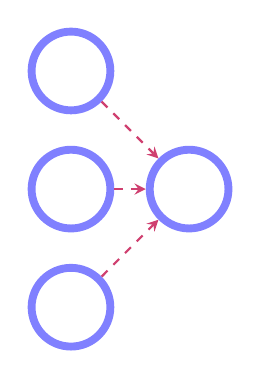
\begin{tikzpicture}[x=1.5cm,y=-1.5cm]
			\node[draw=blue!50,line width=1mm,circle,minimum size=1cm] (n1) at (0,0) {};
			\node[draw=blue!50,line width=1mm,circle,minimum size=1cm] (n2) at (0,1) {};
			\node[draw=blue!50,line width=1mm,circle,minimum size=1cm] (n3) at (0,2) {};
			\node[draw=blue!50,line width=1mm,circle,minimum size=1cm] (o1) at (1,1) {};
			\foreach \i in {1,2,3}{
					\draw[-stealth,dashed,thick,purple!75] (n\i) -- (o1);
				}
		\end{tikzpicture}
	\end{minipage}
\end{frame}

\subsection{Training}

\begin{frame}
	\centering
	\vfill
	\textbf{\Large Training}
	\vfill
\end{frame}

\begin{frame}
	\frametitle{Training (Cycle)}
	\begin{enumerate}
		\item<+-> Input data \only<5->{\checkmark}
		\item<+-> \only<6>{\color{red}}Run the network\only<6>{?}
		\item<+-> Compare output with expected values

		$\rightarrow$ Calculate error ($\lvert v-\text{expected}\rvert$)
		\item<+-> Run error back through network, adjust weights
	\end{enumerate}
\end{frame}

\begin{frame}
	\frametitle{Run the network}
	\centering
	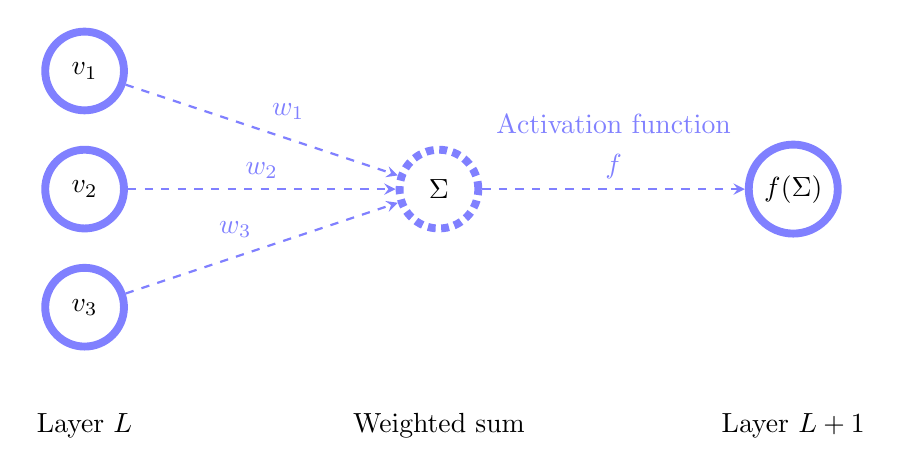
\begin{tikzpicture}[x=4.5cm,y=-1.5cm]
		\tikzset{
			netnode/.style={draw=blue!50,line width=1mm,circle,minimum size=1cm},
		}
		\node[netnode] (i1) at (0,0) {$v_1$};
		\node[netnode] (i2) at (0,1) {$v_2$};
		\node[netnode] (i3) at (0,2) {$v_3$};
		\node[netnode,dotted] (h1) at (1,1) {$\Sigma$};
		\node[netnode] (o1) at (2,1) {$f(\Sigma)$};
		\foreach \i in {1,2,3}{
				\draw[-stealth,dashed,thick,blue!50] (i\i) -- node[auto] {$w_{\i}$} (h1);
			}

		\draw[-stealth,dashed,thick,blue!50] (h1) -- node[auto,label=above:Activation function] {$f$} (o1);
		\node (vl) at (0,3) {Layer $L$};
		\node (sl) at (1,3) {Weighted sum};
		\node (nl) at (2,3) {Layer $L+1$};
	\end{tikzpicture}
\end{frame}

\begin{frame}
	\frametitle{Training (Cycle)}
	\begin{enumerate}
		\item Input data \checkmark
		\item Run the network \checkmark
		\item Compare output with expected values

		      $\rightarrow$ Calculate error ($\lvert v-\text{expected}\rvert$) \only<2->{\checkmark}
		\item \only<3>{\color{red}}Run error back through network, adjust weights\only<3>{?}
	\end{enumerate}
\end{frame}

\begin{frame}
	\frametitle{Adjusting weights}

	\begin{block}{Backpropagation}
		Calculate change of error when adjusting some weight

		$\rightarrow$ \emph{Slope}
	\end{block}\bigskip

	\begin{center}
		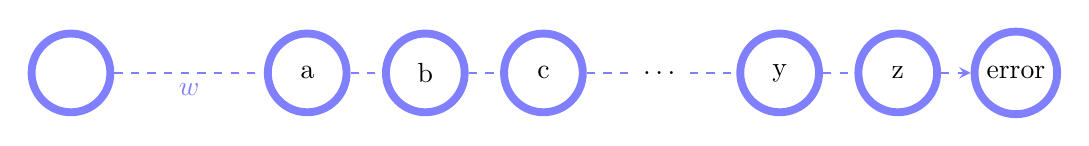
\begin{tikzpicture}[x=1.5cm]
			\tikzset{
				netnode/.style={draw=blue!50,line width=1mm,circle,minimum size=1cm},
			}
			\node[netnode] (s) at (-1,0) {};
			\node[netnode] (a) at (1,0) {a};
			\node[netnode] (b) at (2,0) {b};
			\node[netnode] (c) at (3,0) {c};
			\node (d) at (4,0) {\dots};
			\node[netnode] (y) at (5,0) {y};
			\node[netnode] (z) at (6,0) {z};
			\node[netnode] (error) at (7,0) {error};

			\draw[-stealth,blue!50,dashed,thick]
			(s) -- node[below] {$w$} (a) -- (b) -- (c) -- (d) -- (y) -- (z) -- (error);
		\end{tikzpicture}
	\end{center}

	\uncover<2->{
		\begin{block}{Chain rule}
			\begin{equation*}
				\frac{\delta\text{error}}{\delta w} = \frac{\delta a}{\delta w} \cdot \frac{\delta b}{\delta a} \cdot \frac{\delta c}{\delta b} \cdot \dots \cdot \frac{\delta z}{\delta y} \cdot \frac{\delta\text{error}}{\delta z}
			\end{equation*}
		\end{block}
	}
\end{frame}

\subsection{Pytorch}

\begin{frame}
	\centering
	\vfill
	\textbf{\Large Pytorch}
	\vfill
\end{frame}

\begin{frame}
	\frametitle{Pytorch}

	\begin{itemize}
		\item Framework for NNs in Python
		\item Easy to use $\rightarrow$ good for testing
		\item works cuda-accelerated
	\end{itemize}

\end{frame}

\begin{frame}
	\centering
	\vfill
	\textbf{\Large Binarized Neural Network}
	\vfill
\end{frame}

\section{BNN Design}

\begin{frame}{Binarisation of Linear Layer}
	\begin{columns}
		\column{0.49\textwidth}
		\begin{itemize}
			\item binarisation of weights
			\item binarisation of input data for hidden layers
			\item calculation through \textit{nn.linear}
		\end{itemize}
		\column{0.49\textwidth}
		\centering
		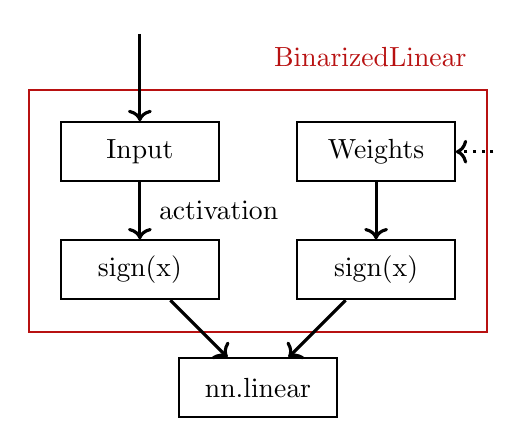
\begin{tikzpicture}[minimum height=0.75cm,minimum width=2cm,line width = 0.25mm]
			\node[rectangle,draw=black] (input) {Input};
			\node[rectangle,draw=black] (weights) at(3,0) {Weights};
			\node[rectangle,draw=black] (sign1) at(0,-1.5)  {sign(x)};
			\node[rectangle,draw=black] (sign2) at(3,-1.5)  {sign(x)};
			\node[rectangle,draw=black] (nnlinear) at(1.5,-3)  {nn.linear};

			\node[scale=0.01] (weightsin) at(4.5,0) {};
			\node[scale=0.01] (inputin) at(0,1.5) {};


			\node[rectangle,draw=preload, fit= (input) (weights) (sign1) (sign2),inner sep=0.4cm] (bnn)   {};
			\node [text=preload,yshift=0.4cm,xshift=-1.5cm] (bnnlabel) at (bnn.north east) {BinarizedLinear};



			\draw [->,dotted,line width = 0.4mm] (weightsin) -- (weights) node[] at(1,-0.75) {activation};
			\draw [->,line width = 0.4mm] (inputin) -- (input);

			\draw [->,line width = 0.4mm] (input) -- (sign1) ;
			\draw [->,line width = 0.4mm] (weights) -- (sign2);

			\draw [->,line width = 0.4mm] (sign1) -- (nnlinear) ;
			\draw [->,line width = 0.4mm] (sign2) -- (nnlinear);


		\end{tikzpicture}

	\end{columns}
\end{frame}


\begin{frame}{Activation}
	Inhalt...
\end{frame}


\begin{frame}{Batch Norm (BN)}
	\begin{itemize}
		\item In NN
		      \begin{itemize}
			      \item normalize batches
			      \item mean 0
			      \item standard derivation 1
		      \end{itemize}
		\item In BNN
		      \begin{itemize}
			      \item prevent \textit{expolding gradient} %TODO graphic
		      \end{itemize}
	\end{itemize}
\end{frame}


\begin{frame}{Evaluation of last layer}
	\begin{columns}
		\column{0.49\textwidth}
		\begin{itemize}
			\item normalisation of activation
			\item decision of the network
		\end{itemize}
		\column{0.49\textwidth}
		\centering
		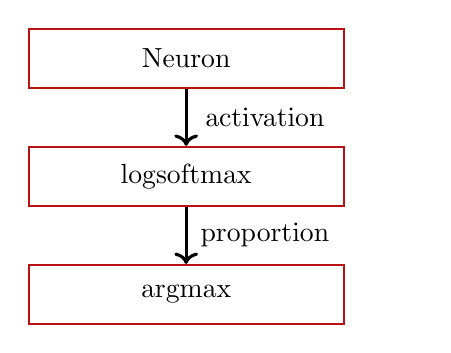
\begin{tikzpicture}[minimum height=0.75cm,minimum width=4cm,line width = 0.25mm]
			\node[rectangle,draw=preload] (neuron) {Neuron};
			\node[rectangle,draw=preload] (softm) at(0,-1.5) {logsoftmax};
			\node[rectangle,draw=preload] (argm) at(0,-3)  {argmax};

			\draw [->,line width = 0.4mm] (neuron) -- (softm) node[] at(1,-0.75) {activation};
			\draw [->,line width = 0.4mm] (softm) -- (argm) node[] at(1,-2.25) {proportion};
		\end{tikzpicture}

	\end{columns}
\end{frame}

\subsection{Binarization of Input data}

\begin{frame}
	\centering
	\vfill
	\textbf{\Large Binarization of Input data}
	\vfill
\end{frame}

\begin{frame}{Binarization of Input data}
	\begin{itemize}
		\item Mapping 255 values to 0,1
		\item minimize accuracy losses
		\item 2 approaches
		\begin{itemize}
			 \item Threshold
			 \item Probability
		\end{itemize}
	\end{itemize}
\end{frame}

\begin{frame}{Threshold-Binarization}
	\begin{columns}
		\column{0.49\textwidth}
		\begin{itemize}
			\item define static threshold
			\item filter pixel-array via: \\pixel $>$ threshold
		\end{itemize}
		\column{0.49\textwidth}
		\centering
  		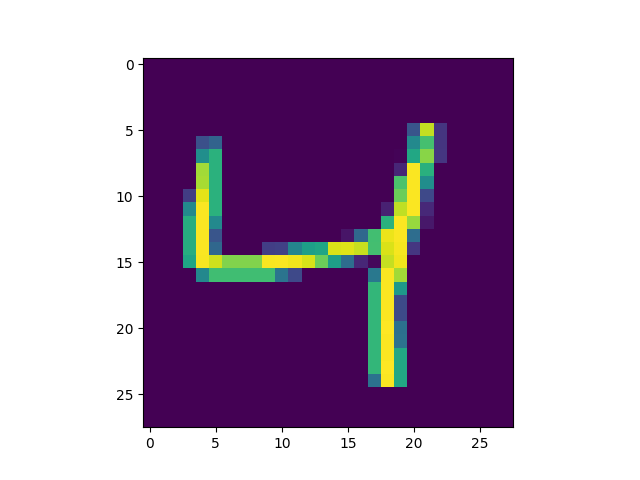
\includegraphics[width=.6\linewidth]{./images/comparison/default}
  		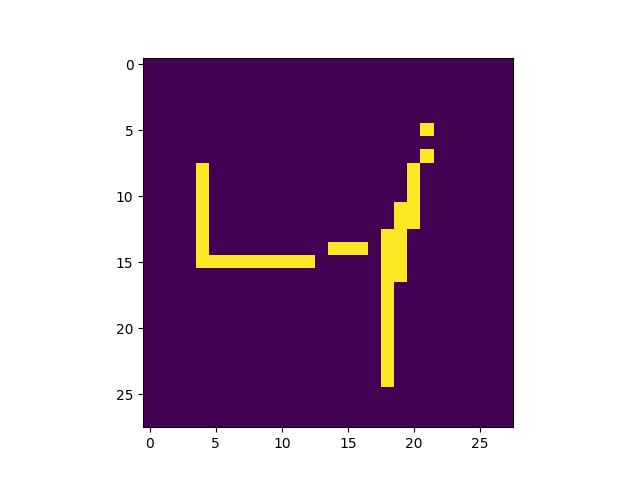
\includegraphics[width=.6\linewidth]{./images/comparison/threshold/200}

	\end{columns}
\end{frame}

\begin{frame}{Probability-Binarization}
	\begin{columns}
		\column{0.49\textwidth}
		\begin{itemize}
			\item each pixelvalue dictates its prob for being 1
			\item binarize same trainingset multiple times
			\begin{itemize}
				\item Run each epoche with all trainingsets
			\end{itemize}
		\end{itemize}
		\column{0.49\textwidth}
		\centering
  		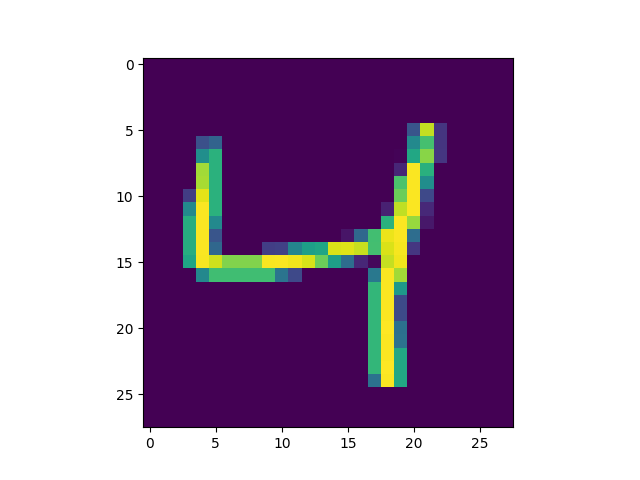
\includegraphics[width=.6\linewidth]{./images/comparison/default}
  		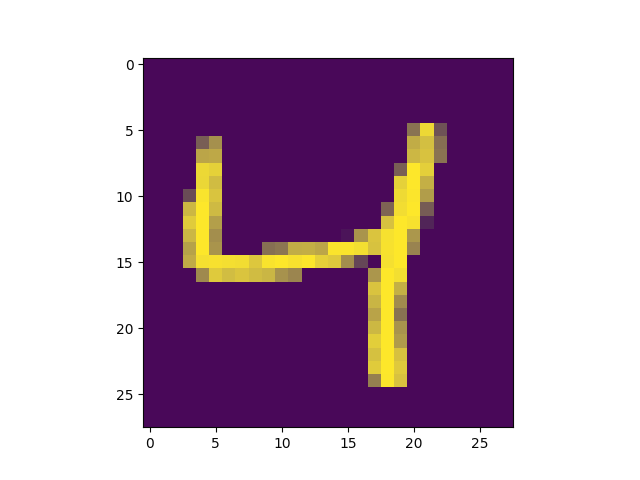
\includegraphics[width=.6\linewidth]{./images/comparison/overlapped}

	\end{columns}
\end{frame}

\begin{frame}{Comparison Threshold, Prob}
	\begin{columns}
		\column{0.49\textwidth}
		\begin{itemize}
			\item Threshold
			\begin{itemize}
				\item Using integrated tensor-functions
				\item 150ms per iteration
				\item Convergence after approx. 100 epochs
			\end{itemize}
		\end{itemize}
		\column{0.49\textwidth}
		\begin{itemize}
			\item Probability
			\begin{itemize}
				\item Iterate through tensor manually
				\item 250ms per iteration
				\item Convergence after approx. 20*30 iterations
			\end{itemize}
		\end{itemize}
		

	\end{columns}
\end{frame}

\begin{frame}{Evaluating Accuracy-Loss}
	\begin{columns}
		\column{0.49\textwidth}
		\centering
		\begin{tabular}{|c|c|c|c|}\hline
			Run & Non-Binarized    & threshold        & prob              \\\hline
			1   	& 91.99\%          & 89.24\%          & 92.52\%           \\\hline
			2   & 91.99\%          & 89.24\%          & 91.82\%           \\\hline
			3   & 91.99\%          & 89.24\%          & 92.56\%           \\\hline
			4   & 91.99\%          & 89.24\%          & 91.02\%           \\\hline
			avg & \textbf{91.99\%} & \textbf{89.24\%} & \textbf{91.98\%}  \\\hline
		\end{tabular}
		\column{0.49\textwidth}
		\centering
		\begin{itemize}
			\item 600 epochs for threshold, default
			\item 20 epochs, 30 trainingsets for prob
		\end{itemize}
	\end{columns}
\end{frame}


\section{BNN Training Analysis}
\begin{frame}
	\tableofcontents[currentsection]
\end{frame}
\subsection{Layer Analysis}
\begin{frame}{Consequences of linear layer binarisation}


	\begin{columns}
		\column{0.49\textwidth}
		\centering
		\begin{tabular}{|c|c|c|}\hline
			Run & binary           & normal           \\\hline
			1   & \textbf{88.29}\% & \textbf{97.43}\% \\\hline
			2   & 87.32\%          & 96.98\%          \\\hline
			3   & 87.19\%          & 97.2\%           \\\hline
		\end{tabular}
		\column{0.49\textwidth}
		\begin{itemize}
			\item training for 50 epochs
			\item mean loss of 9,6\%
			\item loss in granularity
		\end{itemize}

	\end{columns}


\end{frame}

\begin{frame}{Effect of Batch Norm}
	\begin{columns}
		\column{0.49\textwidth}
		\begin{itemize}
			\item 7.4\% improved peak performance
			\item Less jitter with BN
			\item Reduced expolding gradient
		\end{itemize}

		\column{0.49\textwidth}
		\centering
		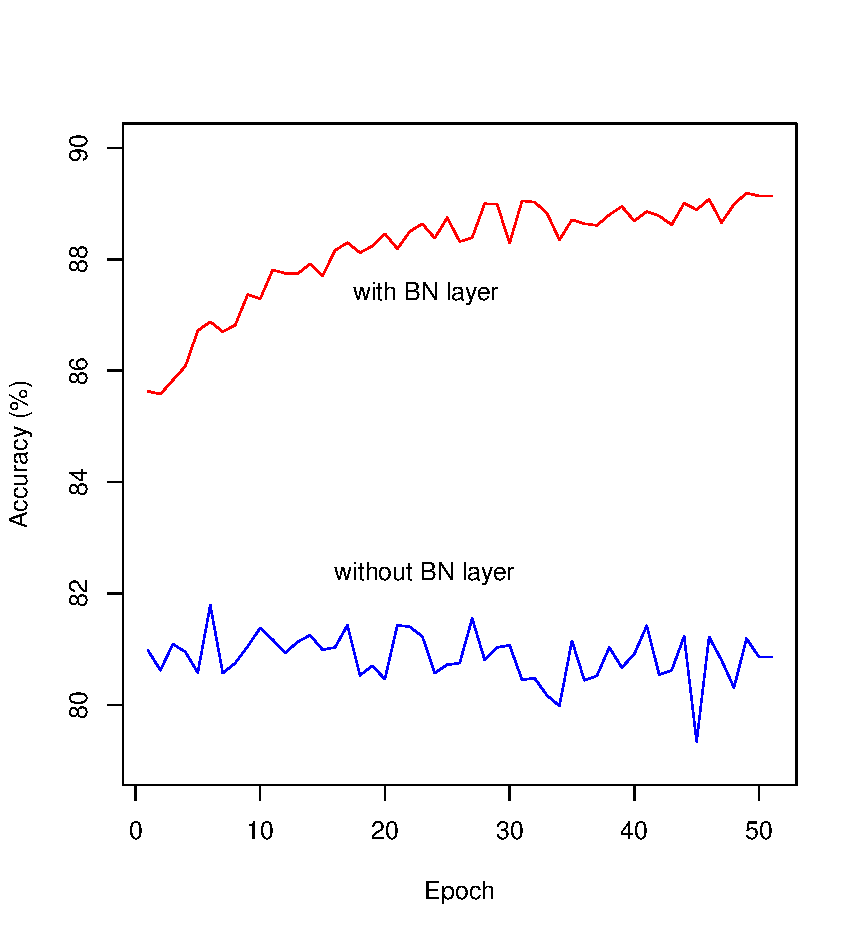
\includegraphics[scale=0.45]{images/batchnorm_measurement.pdf}
	\end{columns}
\end{frame}


\subsection{Parameter Analysis}
\begin{frame}{learning rate}
	\begin{columns}
		\column{0.49\textwidth}
		\begin{itemize}
			\item higher value $\rightarrow$ more weights are updated
			\item balance between over- and underfitting
		\end{itemize}
		\column{0.49\textwidth}
		%TODO Graph over- and underfitting



	\end{columns}

\end{frame}
\begin{frame}{evaluation learning rate}
	\centering
	\vspace*{-1cm}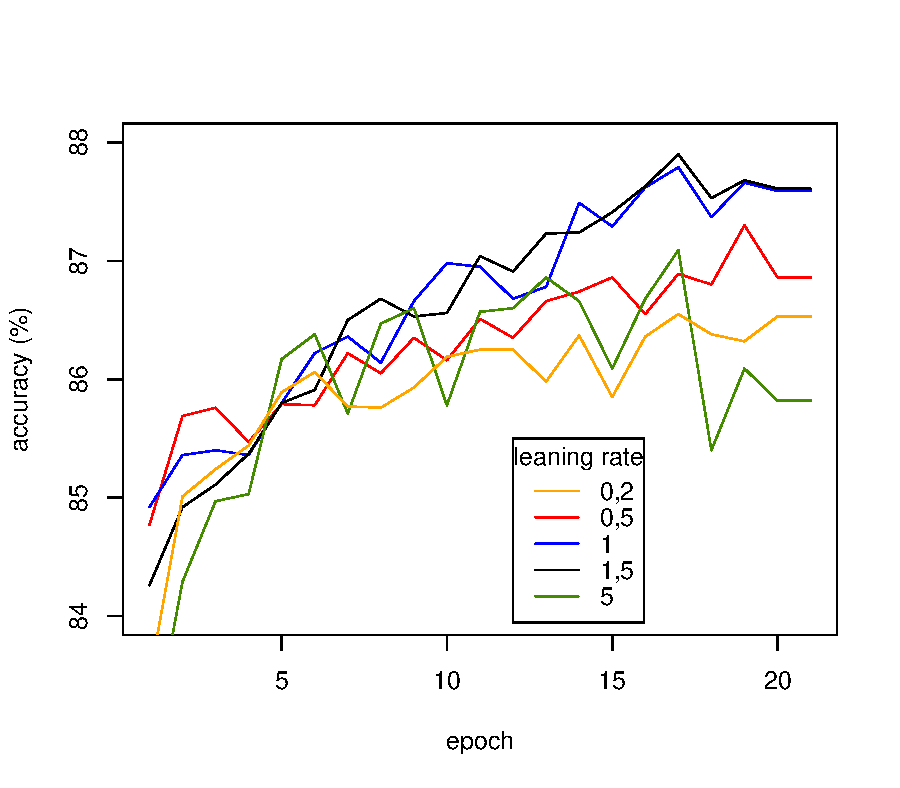
\includegraphics[scale=0.6]{images/learningrate_measurement.pdf}
\end{frame}






\end{document}
